\documentclass{llncs}
\usepackage{makeidx}
\usepackage[english]{babel}
\usepackage[utf8]{inputenc}
\usepackage{amsmath}
\usepackage{url}
\usepackage{fancyvrb}
\usepackage[spanish]{babelbib}
\usepackage{graphicx}


%%%%%%%%%% Text with box
\usepackage{tikz}
\usetikzlibrary{shadows}

\newcommand{\raisedtext}[1]{
  \vspace{2mm}
  \begin{tikzpicture}
    [baseline=(X.base)]\node [drop shadow,fill=white,draw,very thin] (X) {#1};
  \end{tikzpicture}
  \vspace{2mm}
}
%%%%%%%%%%%%%%%%%%%



\graphicspath{ {img/} }

\urldef{\mails}\path|{fbarrios,fjlopez}@fi.uba.ar| 

\newtheorem{definicion}{Definition} 

\begin{document}

\frontmatter

\title{Variations of TextRank for Automated Summarization}
\titlerunning{Variantes de TextRank} 


\maketitle

\begin{abstract}
This article describes our proposal for new variants of the TextRank algorithm for automated summarization of texts. We describe the generalities of the TextRank algorithm on its original version and the different variations of the algorithm that we created. Some of these variants achieve a significative improvement over the original algorithm using the same metrics and dataset as the original publication. 
\keywords{TextRank, summary, automated}

\end{abstract}

\section{Introduction}
We can describe the process of automated summarization as the extraction of the most important sentences in a document. Using different levels of compression a summarized version of the document of arbitrary length can be obtained. The TexRank algorithm is one of the most used methods for this task. TextRank builds a graph of sentendes for a document and then applies PageRank to obtain a score for each sentence. The sentences with higher score are then used for the summary presented in the order in which they appear in the text. Using different schemes for the construction of the graph we can achieve different results. In this article we describe several different proposals for the construction of the TextRank graph and report the results obtained with them.

The first section of this article describes previous work in the area and the TextRank algorithm in general. Then we describe the different metrics used for the evaluation of the results obtained from the proposed changes and the datasets used for these tests. Finally we report the results obtained for the different variations of the algorithm.

\section{Previous work}
The field of automated summarization has advanced in a significative way since the late 60's 
\cite{miranda}. Traditional methods for text summarization analyze the frequency of words or sentences in the first paragraphs of the text to identify the most important ones. Several statistical models have been developed based on training corpuses to combine different heuristics using keywords, position and length of sentences, word frequency and titles \cite{hovy}. Other methods are based in the representation of the text as a graph: the most important sentences are the most connected ones in the graph and are used for the summarization \cite{barzilay}. On a different approach some algorithms analyze the semantic structure of the different textual units in a document with the goal of sepparating those that take a significative role in the representation of the document \cite{marcu}.

The algorithms based on the construction of a graph to represent text used different information retrieval techniques to identify similar sentences and determine the most important ones to build a final summary \cite{salton}. The algorithms developed by Mihalcea and Tarau on TextRank \cite{mihalcea-tarau} and also by Erkan and Radev on LexRank \cite{erkan} are based in ranking the lexical units of the text (sentences or words).

\section{TextRank}

\subsection{Description}
TextRank is an unsupervised algorithm based in graphs for the automated summarization of texts that can also be used to obtain the most important keywords in a document. It was introduced in 2004 by Rada Mihalcea and Paul Tarau on their paper “TextRank: Bringing Order into Texts” \cite{mihalcea-tarau}.

The algorithm applies a variation of PageRank \cite{pageetal98} over a graph constructed specifically for the task of summarization. This method allows to understand the structure of the document identifying its principal concepts without the need of previous training. Since the algorithm is based on PageRank it uses the idea of ranking of the elements in the graph, the most important elements are the ones that better describe the text. This approach allows TextRank to build summaries without the need of a training corpus or labeling and allows the use of the algorithm in different languages as long as there is a way to build the graph of sentences for it.

\subsection{Text as a Graph}
TextRank models any document as a graph, it can use words or sentences as the different nodes in the graph. Sentences are used for automated summarization and words for keyword extraction. After extracting sentences as nodes in a graph the algorithm needs to build edges in between. A function to compute the simmilarity of sentences is then needed. The simmilarity function is used to weight the graph edges, the higher the simmilarity between sentences the more important the edge between them will be in the graph. In the domain of a Random Walker as used frequently in PageRank we can say that we are more likely to go from one sentence to another if those sentences are very similar. 

The simmilarity function can use several different ideas, it can be based in the semantic of the sentences, in their proximity in the text, common words, and many other different metrics. The idea of this article is to experiment with different simmilarity functions and report the results obtained when used along with TextRank.


\subsection{Automatic Summarization}
The problem can be seen as the extraction of the most significative sentences in the document. In this work the lexical units used for the algorithm will be complete sentences \cite{introductionir}.

The simmilarity function used between sentences (nodes in the graph) can be formalized as:


\begin{definicion}
Given $S_i$, $S_j$ two sentences represented by a set of $n$ words that in 
$S_i$ are represented as $S_i = w_{1}^{i}, w_{2}^{i},..., w_{n}^{i}$. The similarity function for $S_i$, $S_j$ can be defined as:


\begin{equation}
Sim(S_{i},S_{j}) = \frac{ | \{   w_{k} | w_{k} \in S_{i} \& w_{k} \in S_{j}   \}  | }    
                              {  log(|S_{i}|) + log(|S_{j}|)  }
\end{equation}


\end{definicion}

The result of this process is a dense graph representing the document. From this graph PageRank is used to compute the importance of each vertex. 

The most significative sentences according to PageRank are selected as the summarization of the text and presented in the same order as they appear in the document.

\section{Example}
A sample document from the 2002 DUC (Document Understanding Conference) dataset is shown next \cite{duc2002-guidelines}:

% \noindent\fbox{%
%     \parbox{\textwidth}{%
% {\scriptsize
\raisedtext{{\scriptsize \parbox{\linewidth}{
\begin{enumerate}
\item Growth Factor Protects Heart Following Attack, Study In Rats Shows 
\item By PAUL RECER AP Science Writer WASHINGTON (AP) 
\item A natural substance called transforming growth factor beta appears to be able to limit damage to cardiac cells following a heart attack, according to a study published in the journal Science.
\item In a study at the Jefferson Medical College in Philadelphia, a group of laboratory rats induced to have heart attacks suffered 50 percent less cell damage after injections of transforming growth factor beta than did rats that did not receive the TGF beta.
\item "TGF beta is a growth factor that opposes some of the bad guys following a heart attack," said Dr. Allan Lefer, a professor at Jefferson.
\item Lefer said his research team simulated heart attacks in 24 rats by partially blocking key arteries in their hearts.
\item In 12 of the rats, the researchers injected a placebo.
\item In the other 12, they injected transforming growth factor beta.
\item For those who received the TGF beta, said Lefer, "the damage from the attack was much less severe.
\item There was about 50 percent less injury with TGF beta than without it".
\item The extent of heart cell damage was determined by measuring the amount of creatine kinase in the heart tissue following an attack.
\item Hearts damaged when the blood supply is interrupted, as in a heart attack, tend to lose creatine kinase, said Lefer.
\item Thus, by measuring for the loss of this substance, researchers could determine the amount of heart damage.
\item Lefer said the TGF beta seems to block the action of other substances, such as tumor necrosis factor, that can cause blood vessels to narrow following a heart attack.
\item Narrowed blood vessels carry less oxygen-rich blood to cells and this causes additional injury following a heart attack.
\item TGF beta is normally present in heart cells, but the study published in Science said that it is missing from rat heart cells damaged by a simulated heart attack.
\item Though TGF beta is produced naturally in the body, Lefer said his research team used a substance produced artificially by Genentech, a California biotechnology firm.
\item Lefer said his team is now conducting additional studies with TGF beta and that any experimental treatment of human heart attack victims with the substance is at least a year away.
\item Jefferson Medical College, where the study was done, is part of Thomas Jefferson University in Philadelphia.
\item Science, which published the study, is the journal of the American Association for the Advancement of Science. 
\end{enumerate}
}
}
}

The TextRank algorithm produces the following summary using the graph shown in Figure 1:


% \noindent\fbox{%
%     \parbox{\textwidth}{%
% {\scriptsize
\raisedtext{{\scriptsize \parbox{\linewidth}{A natural substance called transforming growth factor beta appears to be able to limit damage to cardiac cells following a heart attack, according to a study published in the journal Science.
In a study at the Jefferson Medical College in Philadelphia, a group of laboratory rats induced to have heart attacks suffered 50 percent less cell damage after injections of transforming growth factor beta than did rats that did not receive the TGF beta.
Lefer said the TGF beta seems to block the action of other substances, such as tumor necrosis factor, that can cause blood vessels to narrow following a heart attack.
TGF beta is normally present in heart cells, but the study published in Science said that it is missing from rat heart cells damaged by a simulated heart attack.}}}
% \par
% }
%     }%
% }

\begin{figure}[h!]
    \centering
    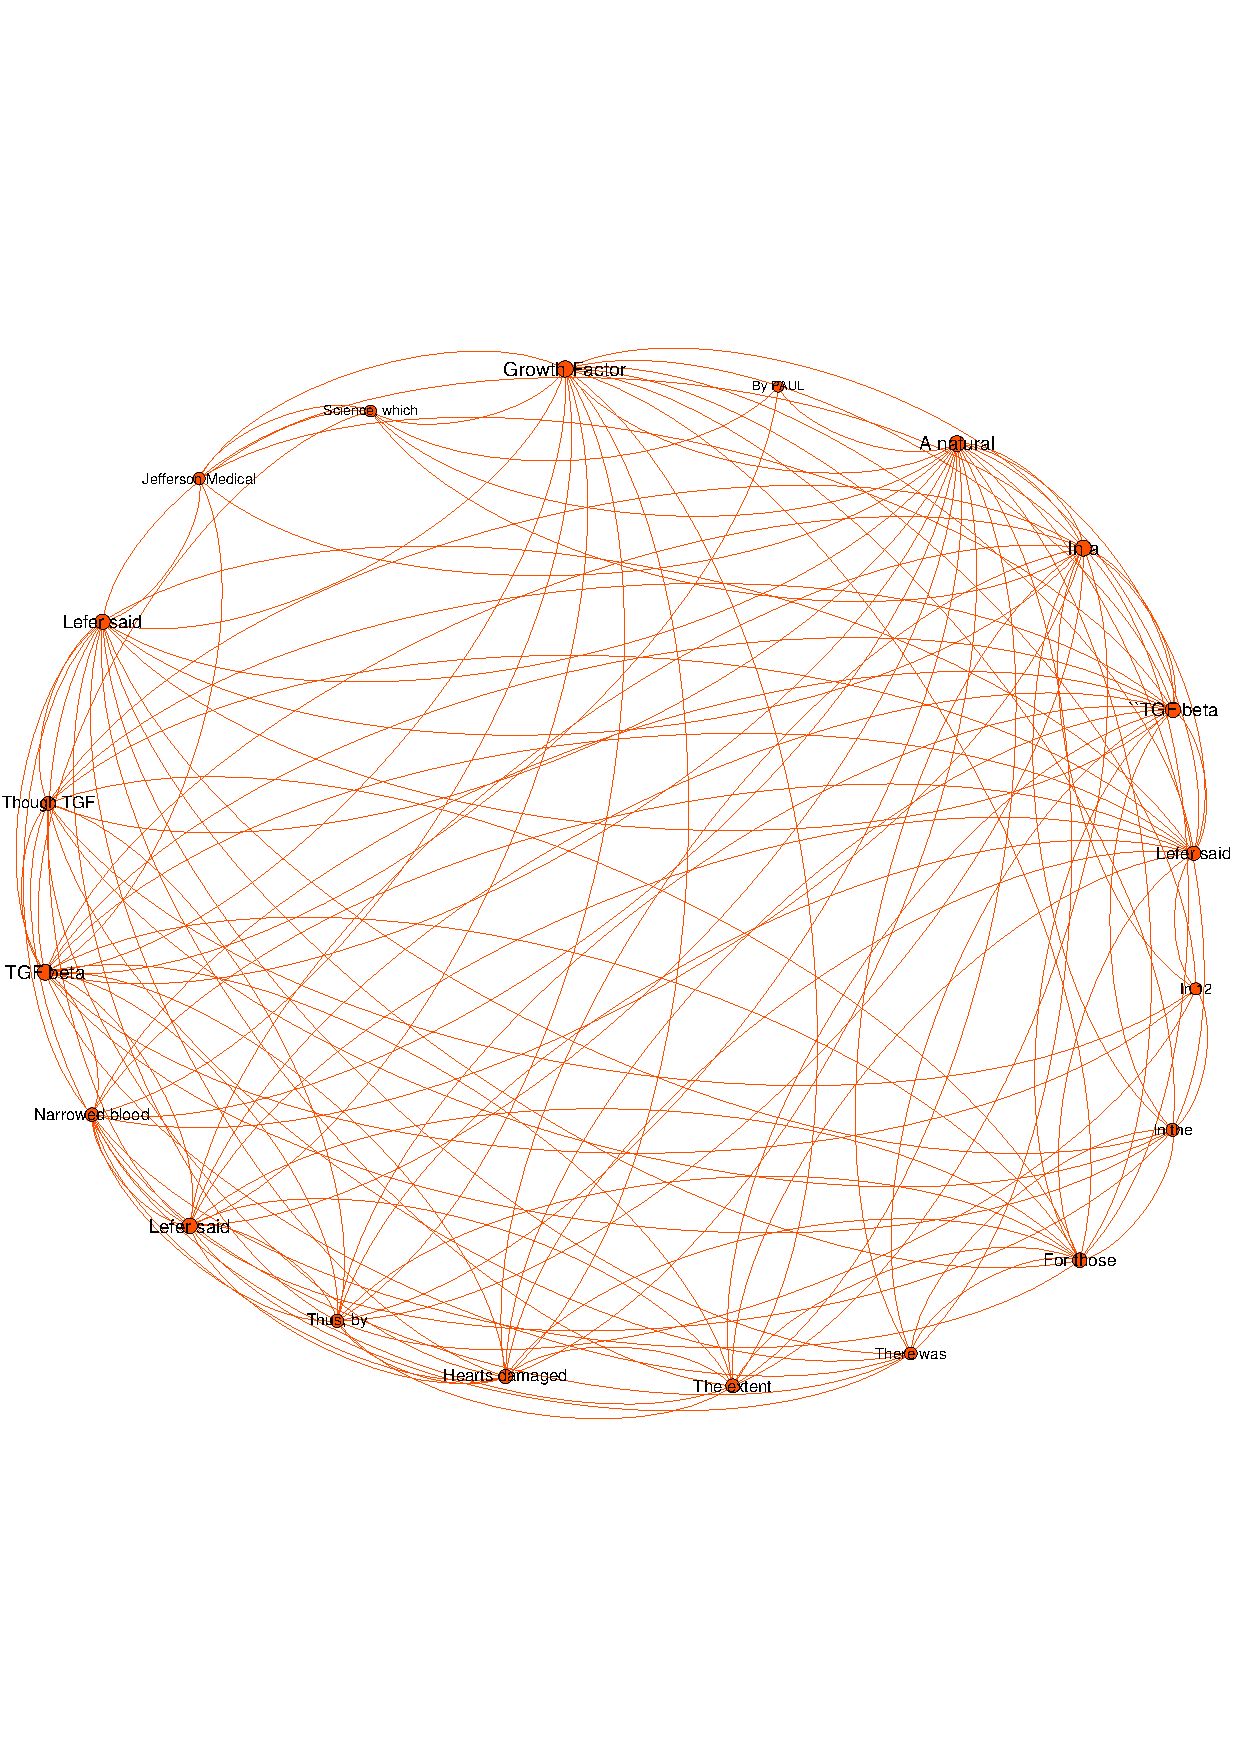
\includegraphics[trim = 0mm 50mm 0mm 50mm, clip, scale=0.15,width=1\textwidth]{graph.pdf}
    \caption{Graph created from the sample text.}
\end{figure}


\section{Experiments}

\subsection{Evaluation}
For testing we used the database of the 2002 DUC (Document Understanding Conference) \cite{duc2002-guidelines} this is the same corpus used in the TextRank original paper in \cite{mihalcea-tarau}. The corpus has 567 documents that are summarized to 20\% of their size.

To evaluate results we used version 1.5.5 of the ROUGE package \cite{Lin2004a}. We used the same configuration used in DUC using ROUGE-1, ROUGE-2 and ROUGE-SU4 as metrics in a 95\% confidence applying stemming. The final result is an average of these three scores.

To check the correct behaviour of our test suite a reference baseline method was used, the same used in \cite{mihalcea-tarau} which is based in the first sentences of each document. We reproduced the results of the standard TextRank Algorithm and found them identical to those reported in the the TextRank paper, a 2.3\% improvement over the baseline.


\subsection{Our Variations}
This sectoin will describe the different variations that we propose over the original TextRank algorithm. These ideas are based in changing the way in which distances between sentences are computed to weight the edges of the graph used for PageRank. We found some of these variations to produce significative improvements over the original algorithm.

\subsubsection{Longest Common Substring}
From two sentences we identify the longest common substring (LCS) and report the simmilarity to be the length of the LCS. This metric is similar to the evaluation methods used in ROUGE.

\subsubsection{Cosine Distance}
The cosine similarity is a metric widely used to compare texts represented as vectors. We used a classical TF-IDF model to represent the documents as vectors and computed the cosine between vectors as a measure of similarity. Since the vectors are defined to be positive the cosine results in values in the range [0,1] where a value of 0 represents identical vectors and 1 represents orthogonal vectors. The cosine similarity can be computed as 1 minus the cosine distance between vectors. 

\subsubsection{BM25}
BM25 / Okapi-BM25 is a ranking function widely used as the state of the art for Informaion Retrieval tasks. BM25 is a variation of the TF-IDF model using a probabilistic model.

\begin{definicion}
Given two sentences R, S, BM25 is defined as:

\begin{equation}
BM25(R,S) = \sum_{i=1}^{n} IDF(s_i) \cdot \frac{f(s_i, R) \cdot (k_1 + 1)}{f(s_i, R) + k_1 \cdot (1 - b + b \cdot \frac{|R|}{avgDL})}
\end{equation}

where $k$ y $b$ are parameters. We used $k = 1,2$ and $b = 0,75$,  $avgDL$ is the average length of the sentences in our collection.
\end{definicion}

In the way this function is defined a word appearing in more than half the documents of the collection will have a negative value. Since this can be a negative effect we used the following correction formula:
                
\begin{equation}
 IDF(q_i) =
  \begin{cases}
       log(N - n(q_i) + 0.5) - log(n(q_i) + 0.5)    & \text{if }  n(q_i) > N/2\\
       \varepsilon \cdot avgIDF                     & \text{if }  n(q_i) \leq N/2\\
  \end{cases}
\end{equation}                
                
where $\varepsilon$ takes a value between 0,5 y 0,30 and $avgIDF$ is the average IDF for all terms.

We also used BM25+, a variation of BM25 that changes the way long documents are penalized.

\subsection{Results}
We tested LCS, Cosine Sim, BM25 and BM25+ as different ways to weight the edges for the TextRank graph. 
The best results were obtained using BM25 and BM25+. The best result was 2.92\% above the original TextRank result using BM25 and $\varepsilon$ = 0.25. The following chart shows the results obtained for the different variations we proposed.

\begin{table}
\caption{Results}
\begin{center}
\begin{tabular}{l*{5}{c}r}
\hline
\rule{0pt}{12pt}
Method & ROUGE-1 & ROUGE-2 & ROUGE-SU4 & Improvement \\[2pt]
\hline\rule{0pt}{12pt}\mbox{}\par\nobreak
BM25 (Neg to epsilon) & 0.4042 & 0.1831 & 0.2018 & 2,92\% \\
BM25+ (Neg to epsilon) & 0.404 & 0.1818 & 0.2008 & 2,60\% \\
Cosine TF-IDF & 0.4108 & 0.177 & 0.1984 & 2,54\% \\
BM25+ (IDF = log(N/NI)) & 0.4022 & 0.1805 & 0.1997 & 2,05\% \\ 
BM25 (IDF = log(N/NI)) & 0.4012 & 0.1808 & 0.1998 & 1,97\% \\ 
Longest Common Substring & 0.402 & 0.1783 & 0.1971 & 1,40\% \\
BM25+ (Neg to zero) & 0.3992 & 0.1803 & 0.1976 & 1,36\% \\ 
BM25 (Neg to zero) & 0.3991 & 0.1778 & 0.1966 & 0,89\% \\
\textbf{TextRank} & \textbf{0.3983} & \textbf{0.1762} & \textbf{0.1948} & \textbf{--}\\
BM25 & 0.3916 & 0.1725 & 0.1906 & -1,57\% \\
BM25+ & 0.3903 & 0.1711 & 0.1894 & -2,07\% \\
DUC Baseline & 0.39 & 0.1689 & 0.186 & -2,84\% \\ [2pt]
\hline
\end{tabular}
\end{center}
\end{table}

The performance in time was also improved. We could process the 567 documents from the DUC2002 database in 84\% of the time needed in the original version.

The result of Cosine Similarity was also satisfactory with a 2.54\% improvement over the original method. The LCS variation also improved the original TextRank algorithm with 1.40\% total improvement.

\begin{figure}[h!]
    \centering
    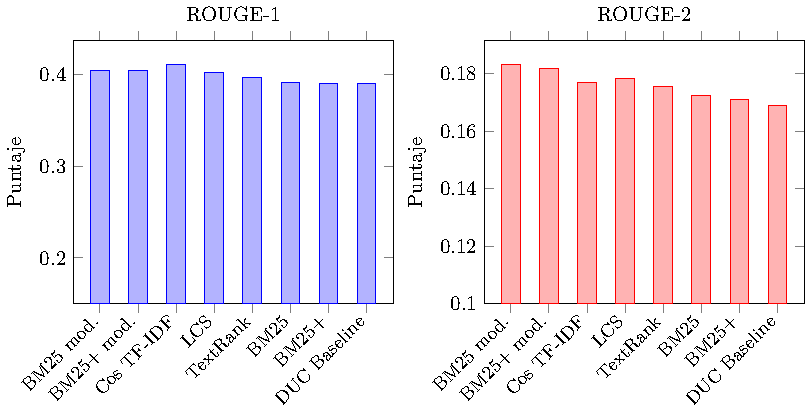
\includegraphics[width=1\textwidth]{rouge-scores.pdf}
    \caption{Comparison.}
\end{figure}

\section{Reference Implementations and Gensim Contribution}
A reference implementation of our proposals was coded as a Python module. It can be obtained for testing and to reproduce results from the following URL: \url{https://pypi.python.org/pypi/summa/0.0.6}.

We also contributed the BM25-TextRank algorithm to the Gensim project. Gensim is a collection of text processing tools in Python designed to be efficient and scalable. Since Gensin didn't have an automated summarization module we contributed our work to the project. 

Gensim can be found at: \url{https://radimrehurek.com/gensim/}.

\section{Conclusions}
This work presented three different variations to the TextRank algorithm for automatic summarization. The three variations presented improved significantly the results of the algorithm using the same metric and database used in the original paper. Given that TextRank performs 2.84\% over the baseline our improvement of 2.92\% over the TextRank result is an important result. 

The combination of TextRank with modern Informatio Retrieval ranking functions such as BM25 and BM25+ results in the creation of a robust method for automatic summarization that performs better than the stadard methods used previously. 

Based on this results we suggest the use of BM25 along with TextRank for the task of unsupervised automatic summarization of texts. The results obtained and the examples analyzed show that this variation is better than the original TextRank algorithm without a performance penalty.
\bibliography{report-en}{}
\bibliographystyle{babunsrt}


\end{document}
